\documentclass[12pt,addpoints]{guia}
\grado{2$^\circ$ de Secundaria}
\cicloescolar{2022-2023}
\materia{Ciencias y Tecnología: Física}
\guia{9}
\unidad{3}
\title{Expansión del universo}
\aprendizajes{\item Describe cómo se lleva a cabo la exploración de los cuerpos celestes por medio de la detección
de las ondas electromagnéticas que emiten.\item Describe algunos avances en las características
y composición del Universo (estrellas, galaxias y otros sistemas).}
\author{JC Melchor Pinto}
\begin{document}
\INFO%
\begin{sectionbox}{Recesión en de las galaxias}
    \begin{wrapfigure}[25]{l}[1mm]{0.55\textwidth}
        \centering
        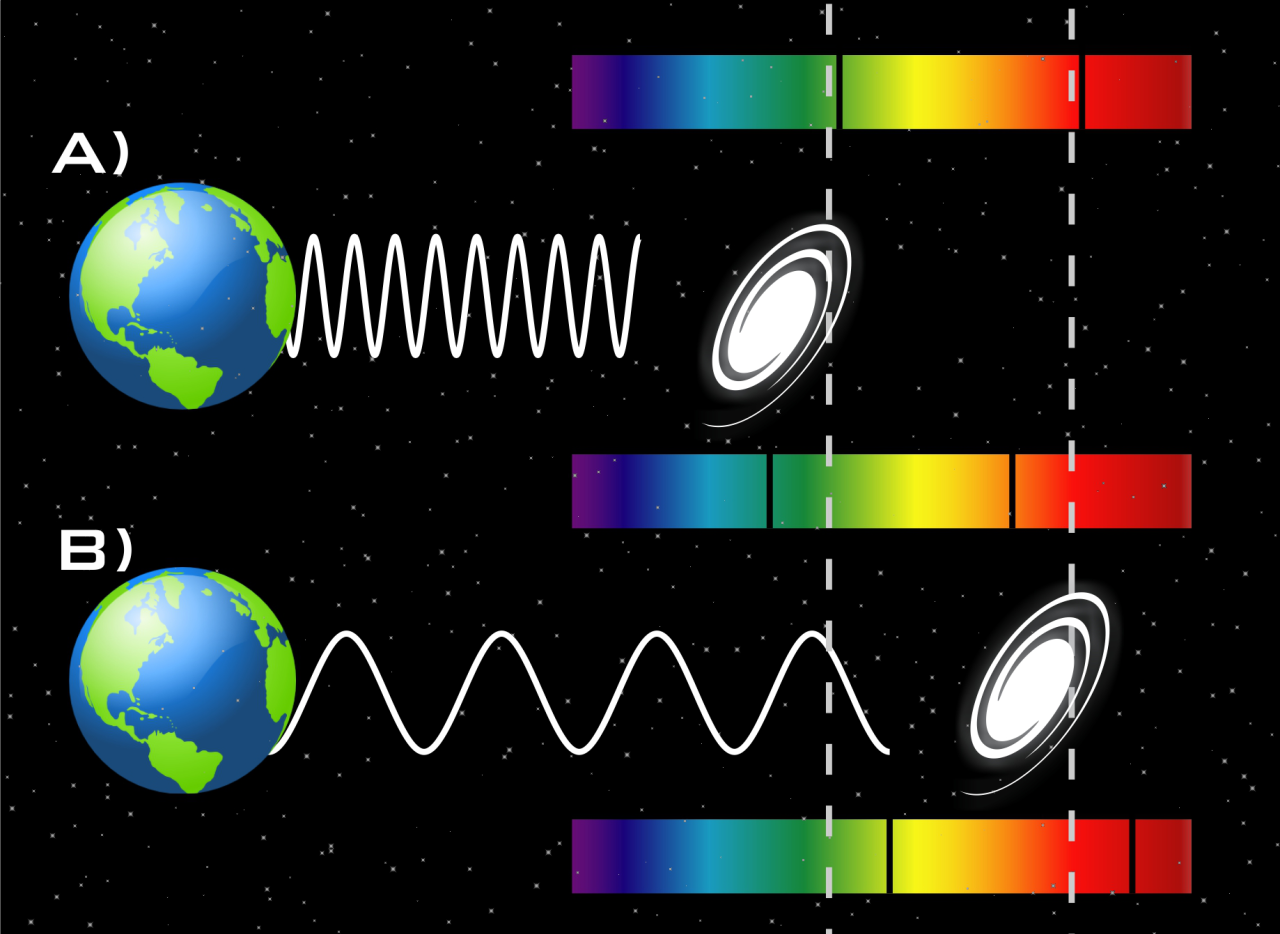
\includegraphics[width=\linewidth]{../images/tumblr_n7luwbd1pO1tf8xldo1_1280}
        \caption{a) Corrimiento Al Azul. Los objetos celestes que se acercan a nosotros presentan sus lineas de absorción recorridas hacia el color azul con respecto a su posición habitual.
            b) Corrimiento Al Rojo. Cuando se alejan de nosotros presentan sus lineas de absorción recorridas hacia el color rojo.}
        \label{fig:tumblr_n7luwbd1pO1tf8xldo1_1280}
    \end{wrapfigure}
    El aspecto mas importante de las galaxias para nuestra comprension del Universo es su recesion\label{086a_a}, es decir, el hecho de que las galaxias se alejan entre si. Hacia 1929 Edwin Hubble y sus colaboradores midieron las distancias y los espectros de la luz de unas 200 galaxias y descubrieron que, en general, mostraban un corrimiento al rojo. Esto significa, si nos basamos en el efecto Doppler (figura \ref{fig:tumblr_n7luwbd1pO1tf8xldo1_1280}) que la longitud de onda de la luz que emitio la galaxia se alargó como consecuencia de su movimiento\label{086b_a} respecto a nosotros, alejandose. La medida de ese alargamiento se conoce como corrimiento al rojo, y se simboliza con la letra z, \label{086a_b}una cantidad importante para describir el Universo.
    El corrimiento al rojo también permitió a
    Hubble determinar que la \label{086b_b}velocidad con la que
    se alejan las galaxias es proporcional a la distancia a la que se encuentran. Esta relación se
    conoce hoy como la \textbf{ley de Hubble}\label{086a_c}.
    La interpretación que se le dio al descubrimiento de Hubble\label{086b_c} es que el Universo se expande, lo
    cual significa que lo que crece es el espacio en
    sí mismo. Esta es la explicación razonable, por
    extraña que parezca, pues de otro modo se diría
    que las galaxias se alejan de la Vía Láctea, como
    si nuestra galaxia estuviera en una posición preferencial.
\end{sectionbox}


\begin{card}[check][Experimenta la expansión del Universo]
    Propósito:
    Construir un modelo que ilustre la expansión del Universo y sus
    efectos físicos.

    Materiales:
    \begin{itemize}
        \item Globo grande,
        \item cuadraditos de papel de 1.5 cm por lado,
        \item cinta adhesiva,
        \item liga ancha.
    \end{itemize}

    Procedimiento:
    \begin{enumerate}
        \item Dibujen galaxias de 1 cm de diámetro en los cuadritos de papel, recórtenlas y
              péguenlas en la superficie del globo un poco inflado. Nuestro universo será
              sólo la superficie del globo. Cuando piensen en distancias para su universo las
              medirán sobre la superficie; elijan una galaxia como referencia.
        \item Uno de ustedes inflará el globo lentamente, mientras el otro observará cómo
              cambia la distancia entre su galaxia y las que la rodean.
        \item Repitan el procedimiento, pero ahora elijan otra galaxia como origen de un
              nuevo sistema de referencia.
        \item Corten la liga, extiéndanla y dibujen el perfil de una onda transversal.
        \item Estiren la liga y observen qué ocurre con la onda.
    \end{enumerate}


    Análisis y conclusiones:
    \begin{itemize}
    \item ¿Al inflar el globo se modela la expansión del Universo como la describe la ley
        de Hubble? Explica.
        \item ¿La liga sirve como modelo del efecto Doppler? ¿Qué cambios observan en la
        onda que dibujaron? ¿En este caso es mejor usar la liga o el globo? Explica.
    \end{itemize}
\end{card}
\begin{questions}
    \questionboxed[50]{\include*{../questions/question086b}}
    \questionboxed[50]{\include*{../questions/question086a}}
\end{questions}
\end{document}